\section{Experimental results}

\subsection{Dataset preprocessing}
The dataset in use is the Illinois Bulk Dataset, that contains 
183146 cases with 194366 judges opinions. 

The first step of the preprocessing is to merge the opinions about a 
case into one, obtaining a single document for each dataset entry.  
Then, each document goes through a text cleaning and tokenization phase, 
where the first part is done with the help of regular expressions, 
while the second uses Spacy to obtain a list of terms.

\subsection{Topic modelling}
To have an overview of the topics discussed on the dataset a Latent 
Dirichlet Allocation model is trained on the tokenized texts.
One of the key parameters of such a model is the number of topics, and, 
given the fact that cases could potentially talk about anything, an 
\emph{Halving search} is performed to find a good value.~\cite{halving-search}

We opt for an halving search since the number of topics could be anything, 
we fixed a range between ten and thirty and training each model 
to then evaluate results would take a huge amount of time. Halving search 
mitigates the problem, as it trains firstly on smaller datasets, select 
the best models, and retrain on bigger slices of data until a final model 
is found. This methodology can be ten times faster then grid search. 
The selection criterium for the search is the Log Likelihood of each model.
The search revealed that the optimal number of topics is 14.

The resulting topics are promising but the words of interest, namely a collection 
of narcotics, investigation and weapons terms, are merged together in a few topics. 
To solve the issue we decide to run topic modelling on a subset of the previous 
topics with the same technique as before. The result is similar, we find again 14 topics, 
but this time they are much more specific.

\subsection{Temporal word embeddings}

One of the objective of the project is to find correlations among words and one tool 
that can be used is word embeddings. The technique assigns a real vector of a given dimensions
to each word in the document collection, creating a way to directly compare the context 
similarity between two terms.

For this task we used Gensim's Word2Vec implementation and trained different models 
in three ways:
\begin{enumerate}
    \item \emph{Global model}: trained on the entire document collection, with 100 components vectors;
    \item \emph{One year models}: they are trained on subsets of the dataset divided by years;
    \item \emph{Ten years models}: trained on epochs of 10 years each.
\end{enumerate}
The first model gives information about the whole dataset, it can be used to compute 
similar words queries, while the others can be exploited to find context and semantic shifts 
among the temporal axis.
Taking inspiration from the HistWords~\cite{hist-words} work on semantic shift, we start by aligning the models, 
and then find, given a word and a base year, the similarity of that word in time with respect 
to the base year. This approach can reveal if a word changed semantic or context, and when, 
with respect to a given year, an example can be seen in \vref{fig1}. 

Similarly, the ten year models are aligned, but this time, given a term, we compute the 
difference among two consecutive epochs. The idea is similar to the previous one but slightly 
different, this time a drop in the similarity sequence 
reveals a change of meaning from an epoch to the other, the resulting 
sequence can be seen in \vref{fig2}.

\begin{figure}
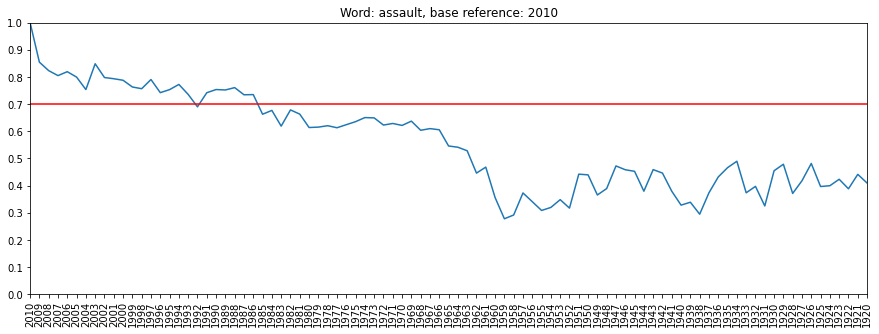
\includegraphics[width=\textwidth]{images/semantic_1.png}
\caption{Semantic shift of the word assault 
with respect to the year 2010, we can see a drop if similarity around 1960.} \label{fig1}
\end{figure}
\begin{figure}
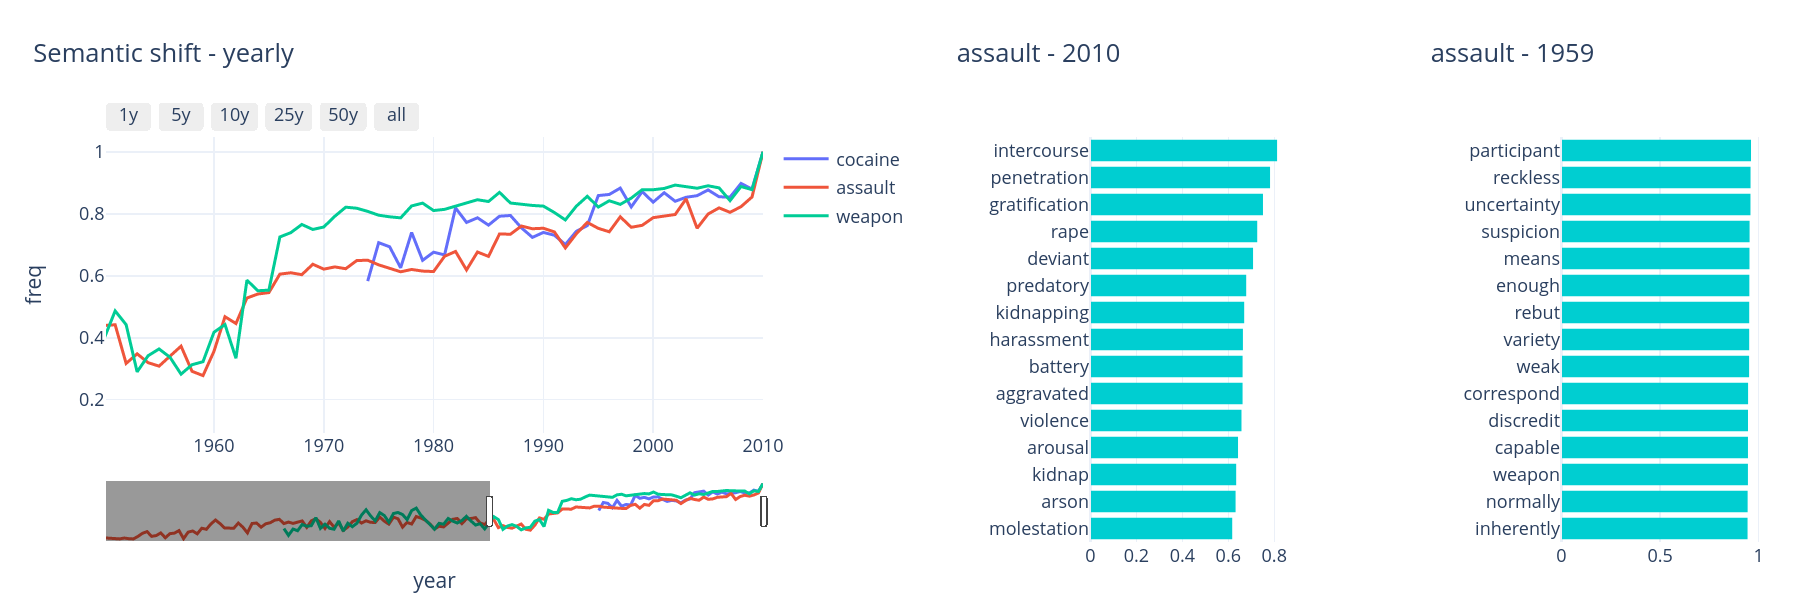
\includegraphics[width=\textwidth]{images/semantic_2.png}
\caption{Similarity between consecutive epochs of the term assault, we can see a 
drop between 1980-1970 and 1970-1960.} \label{fig2}
\end{figure}
\subsection{Webapp}
In order to visualize and explore the results of the analysis, a web interface has been developed. Through the UI, the
user can search multiple words united (separated by ",") and/or confront words (separated by "-"); the app will show
various interesting sections:
\begin{itemize}
  \item Top 15 words of similar context of the searched words (using word embeddings).
  \item Frequency graph of documents in time containing the searched words.
  \item Semantic shifts of the searched words, both by epoch (two adjacent epochs of 10 years) and by single year.
    If the user clicks on a point of the graph, the contexts of the selected word in the different selected years/epochs
    will be showed, allowing the comparison of contexts which helps understanding the evolution of words meaning and usage
    during time.
  \item Topic distribution of the searched words (both generic and areas of interest-specific topics). By clicking on the
    showed radar chart, or on the lateral list of topics, the selected topic info will be loaded in the below section.
  \item Most important words of the selected topic. There are three ways of visualization: a barchart with the first 15
    words, a Wordcloud with the first 80 and a Treemap with the first 50.
  \item Topic distribution over time and over the different Illinois courts.
\end{itemize}
The application has been developed in Python and is accessible at https://illinois-cases-analysis-webapp-qka7d4ktba-ew.a.run.app/ .
\subsubsection{Webapp developing technology}
\subsubsection{Cloud hosting}
